\section{Gripper Stall charts}




\subsection{Current-based overstepping}
\label{app:stall-current-overstepping}

This chart shows a case where the current based stall detection did not stop the motor cleanly at the stall point. The current signal crosses the threshold repeatedly, but the signal is noisy and does not give a clear single transition from normal movement to stall. Because the software had to wait for repeated samples above the threshold, the motor could continue moving for too long before the stall was accepted.

This caused overstepping, where the gripper moved further than intended after reaching the mechanical resistance. This was one of the reasons why current based stall detection was not selected as the final method.

\begin{figure}[H]
    \centering
    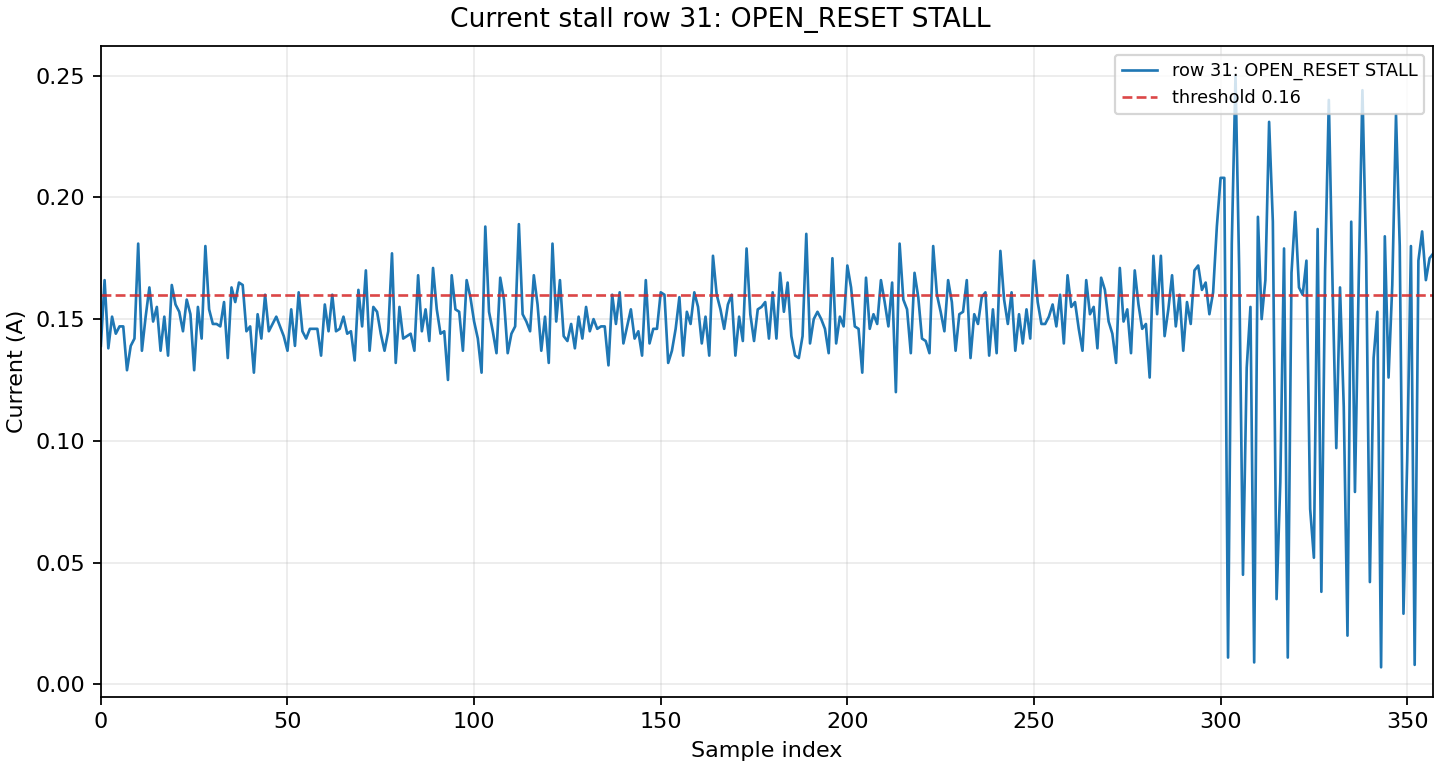
\includegraphics[width=1\textwidth]{Appendix/Images/StallChartOverstepping.png}
    \caption{Current based stall detection with overstepping at stall.}
    \label{fig:stall-chart-with-overstepping}
\end{figure}


\clearpage
\subsection{Stall against hardstop vs. against cube with spring coupling}
\label{app:stall-charts}

The charts show the stall signals recorded during the gripper tests. Both the StallGuard value and the current based stall signal are shown for a hardstop measurement and for gripping an object with the spring coupling extending.

\begin{figure}[H]
    \centering
    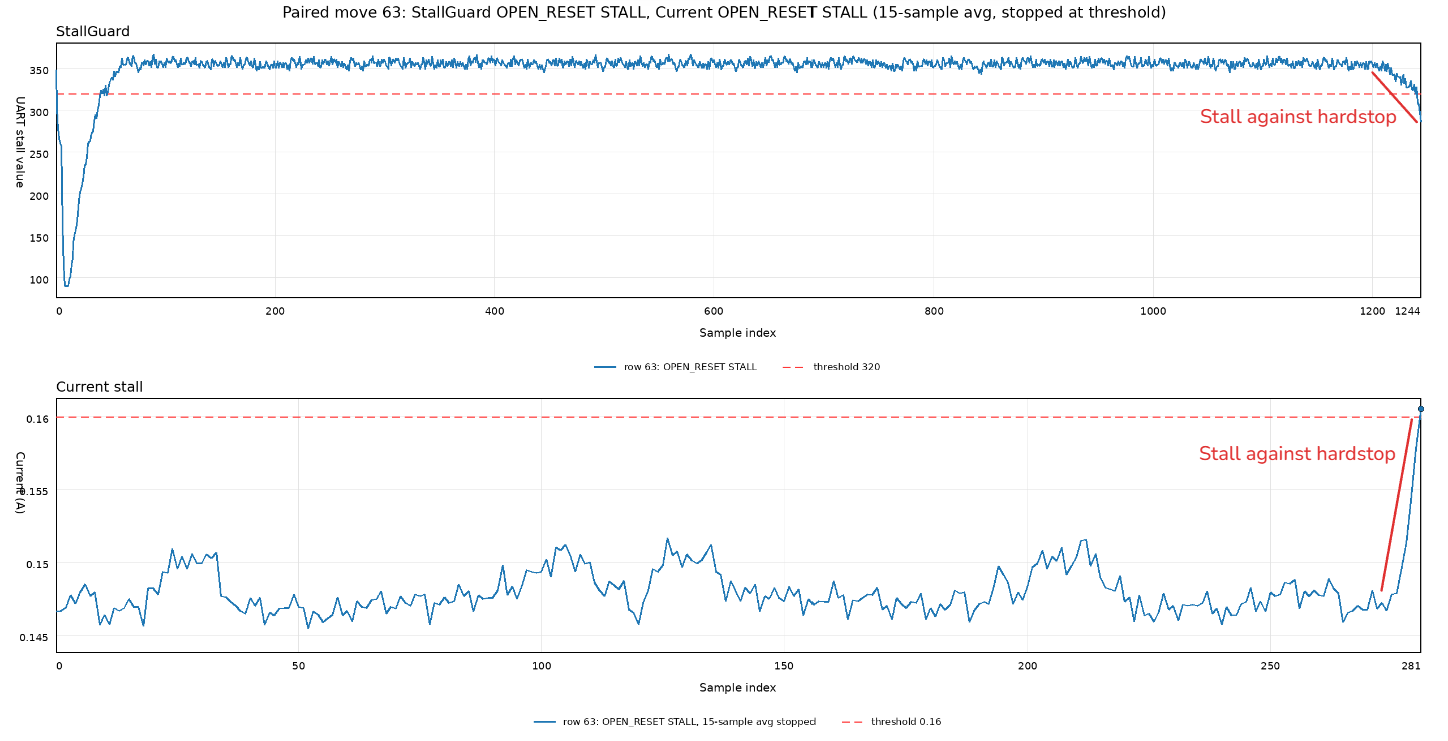
\includegraphics[width=1\textwidth]{Appendix/Images/StallChartHardstop.png}
    \caption{Stall detection measurements when the gripper reaches the hard stop.}
    \label{fig:stall-chart-hard-stop}
\end{figure}

\begin{figure}[H]
    \centering
    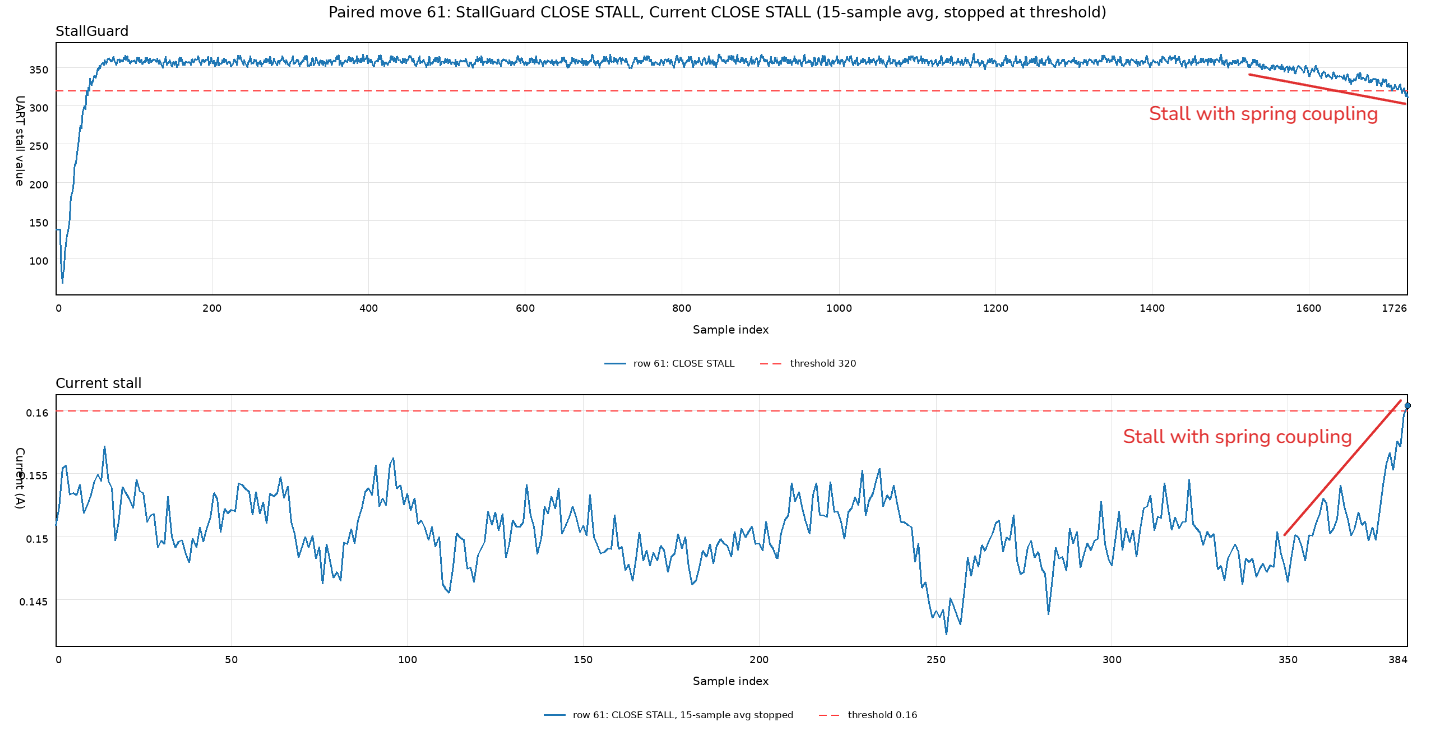
\includegraphics[width=1\textwidth]{Appendix/Images/StallChartWithSpring.png}
    \caption{Stall detection measurements with the spring mechanism.}
    \label{fig:stall-chart-with-spring}
\end{figure}
